\documentclass[usenames,xcolor=dvipsnames]{beamer}
\usecolortheme{orchid}
\usetheme{CambridgeUS}

\title[Insecurely Wrapping Secure Software]{Docker -- Insecurely Wrapping Secure Software.}
\author{Aleksa Sarai}
\institute{\texttt{SYD0x05}}
\date{March 2015}

\usepackage{hyperref}
\hypersetup{pdfpagemode=FullScreen}

\usepackage{graphicx}
\graphicspath{{assets/}}

\usepackage{float}
\usepackage{color}
\usepackage{graphics}
\usepackage{ulem}
\usepackage{textcomp}

% Cash money.
\definecolor{cashgreen}{rgb}{0.0, 0.5, 0.0}

% Define a nice list environment.
\newenvironment{list**}
	{\begin{list}{\textcolor{blue}{$\ast$}}{\leftmargin=1em \itemindent=0em}}
	{\end{list}}

% Define a nice definition environment.
\newenvironment{definition**}
	{\begin{list}{}{\leftmargin=2.5em \itemindent=0em}}
	{\end{list}}

% Define a nice definition environment.
\setbeamertemplate{enumerate items}[default]
\newenvironment{enumerate**}
	{\begin{enumerate}}
	{\end{enumerate}}

% Redefine \sout<> to allow for beamer magic.
\renewcommand<>{\sout}[1]{
  \alt#2{\beameroriginal{\sout}{#1}}{#1}
}

\begin{document}

% Title page.
\begin{frame}
	\titlepage
\end{frame}

% Hack to create a changing title page.
\title[Insecurely Wrapping Secure Software]{}
\subtitle{A short(ish) spiel on how monolitic tools like Docker can create insecure systems through trivial vulnerabilities, especially if they are built atop secure software.}
\begin{frame}[noframenumbering]
	\titlepage
\end{frame}

% Hello page.
\begin{frame}
	\frametitle{\texttt{puts("Hello, s3ct41k5!");}}
	\begin{list**}
		\item<2-> Hello there, I'm Aleksa (aka \texttt{cyphar}).
		\item<3-> I've been interested in hacking Gibsons / writting cool software since I was a young `un.
		\item<4-> More relevant to this talk, I'm a maintainer of and active contributor to Docker (as well as \texttt{libcontainer}).
			\begin{list**}
				\item<5-> \dots which means I have a somewhat unique view of the state of Docker's security.
			\end{list**}
		\item<6-> \textbf{tl;dr}: If you thought that Docker was a cool way to use secure Linux kernel features, think again.
		\item<7-> \textit{Disclaimer}: I don't work for Docker, so anything I say (offensive or otherwise) isn't funded by that sweet, \textit{sweet} Docker money.
	\end{list**}
\end{frame}

% Troll Docker money slide.
\begin{frame}
	\frametitle{Docker money?}
	\begin{figure}[h]
		\centering
		\only<2->{\scalebox{0.8}{
\includegraphics[width=\linewidth]{money}}}
		\only<2->{\caption{``\texttt{1 g0t th4t D0ck3r m0n3y!}''}}
	\end{figure}
\end{frame}

% Intro to Docker.
\begin{frame}
	\frametitle{What is an Docker? How I can haz one?}
	\begin{list**}
		\item<2-> Who's heard of Docker\only<3->{ / used Docker}\only<4->{ / worked on Docker}?
		\item<5-> \sout<6->{Kick-ass new Linux technology that provides trivial (semi-)containerisation, consistent development environments (without the negatives of heavy VMs), makes unicorns real, etc.}
		\begin{list**}
			\item<6-> --- not really, it's more of a wrapper of fairly new-ish Linux kernel technologies (cgroups and Linux namespaces).
		\end{list**}
		\item<7-> The reason why people (including me) rave about Docker so much is because it solves a problem that developers and sysadmins have been trying to solve since time immemorial:
		\begin{list**}
			\item<8-> How \textit{exactly} do you ensure that you can deploy some software anywhere in your datacenter without undergoing dependency hell?
		\end{list**}
	\end{list**}
\end{frame}

% Dummy replacement slide.
\begin{frame}[noframenumbering]
	\frametitle{What is an Docker? How I can haz one?}
	\begin{list**}
		\item<1-> But none of that \textit{really} matters for this talk. All that matters for the purposes of this talk is that Docker is wrapping some pretty damn cool Linux kernel features with a fairly nice interface.
		\item<2-> \dots but I'd be glad to demo it if you like. \texttt{:P}
	\end{list**}
\end{frame}

% Introduce issue.
\begin{frame}
	\frametitle{And herein lies the issue \dots}
	\begin{list**}
		\item<2-> So, what happens if you find a trivial security vulnerability in Docker?
		\item<3-> \textbf{tl;dr}? \only<4->{\texttt{{[}+{]} w00t w00t g0t r00t :).}}
		\item<5-> Why? \only<6->{Because \texttt{/usr/bin/docker} is a daemon on your system running as \texttt{r00t} and provides an API to clients on the system. Vulnerabilities in Docker are vulnerabilities in a long-running \texttt{r00t}-level daemon.}
		\begin{list**}
			\item<7-> Even though the processes are containerised by Linux, if the wrappers are vulnerable the whole system becomes vulnerable.
			\item<8-> {\it Aside: the kernel actually doesn't have any concept of a "container".}
		\end{list**}
		\item<9-> "What vulnerabilities?" I hear you say \dots
	\end{list**}
\end{frame}

% First symlink and path vulnerability.
\begin{frame}
	\frametitle{Symlinks!}
	\begin{list**}
		\item<2-> Everyone loves symlinks, right? \only<3->{\dots \textit{right guys}?}
		\item<4-> Turns out, symlinks are hard.
		\item<5-> Like, \textbf{really} hard.
			\begin{figure}
				\only<5->{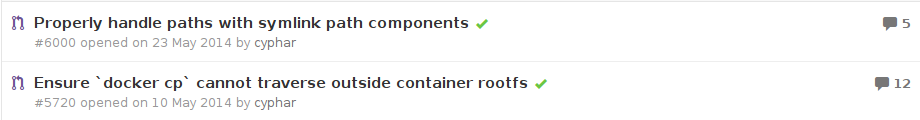
\includegraphics[width=\linewidth]{prlist}}
			\end{figure}
		\item<6-> The above are fixes for \textbf{two} vulnerabilities involving path sanitisation and symlinks.
			\begin{list**}
				\item<7-> They allow you to read \textbf{any} file as though you are \texttt{r00t}.
			\end{list**}
		\item<8-> This vulnerability affects \textcolor{BurntOrange}{\texttt{docker<0.12.0}}, so if you've updated in the last year you're not vulnerable.
	\end{list**}
\end{frame}

% Explanation.
\begin{frame}[noframenumbering]
	\frametitle{Symlinks!}
	\begin{list**}
		\item<1-> So, how did the vulnerability work?
		\item<2-> Docker provides the ability to copy files from a container using the \texttt{docker cp} command.
		\item<3-> However, the container path was not sanitised properly (see: not sanitised \textbf{at all}).
		\item<4-> So the following paths would allow you to copy \texttt{/etc/shadow} from the host filesystem:
			\begin{enumerate**}
				\item<5-> \texttt{../../../../../../../etc/shadow}.
				\item<6-> \texttt{/symlink/shadow} (where \texttt{/symlink} points to \texttt{/etc/}).
				\item<7-> \texttt{/symlink/shadow} (where \texttt{/symlink} points to \texttt{../../../../../../../etc/}).
			\end{enumerate**}
		\item<8-> There were a few others, but for some reason I've been unable to replicate them -- even after \texttt{git bisect}ing the repo.
	\end{list**}
\end{frame}

% Yay, demos!
\begin{frame}
	\center\scalebox{2.5}{Demo!}
\end{frame}

% Second symlink vulnerability.
\begin{frame}
	\frametitle{Moar symlinks! \textcolor{blue}{\texttt{CVE-2014-9356}}.}
	\begin{list**}
		\item<2-> Remember how I said symlinks are hard?
		\item<3-> Well, here's a vulnerability present in \textcolor{BurntOrange}{\texttt{docker<1.3.3}}.
		\item<4-> Turns out that some other features of Docker wouldn't correctly scope symlinks and then you had read-write access to the host filesystem.
		\item<5-> Looks like they didn't learn their lesson the first time \dots
	\end{list**}
\end{frame}

% Explanation.
\begin{frame}[noframenumbering]
	\frametitle{Moar symlinks! \textcolor{blue}{\texttt{CVE-2014-9356}}.}
	\begin{list**}
		\item<1-> So, how did this vulnerability work?
		\item<2-> This was actually a general vulnerability, caused by broken path sanitisation in several places inside \texttt{Dockerfile} evaluation.
		\item<3-> One example of this vulnerability is that the \texttt{VOLUME} instruction would create a new \texttt{VFS} volume, but instructions like \texttt{COPY} would still traverse a symlinked volume path when referencing data in the volume:
			\begin{enumerate**}
				% NOTE: Make sure you highlight this. It's used in the CTF.
				\item<4-> Create a symlink as the volume path pointing to \texttt{/../../../../../../../<path>}.
				\item<5-> Expose the \texttt{VOLUME}.
				\item<6-> \texttt{COPY} any file to the volume and it gets written to \texttt{<path>} on the host.
			\end{enumerate**}
		\item<7-> It was also possible to use \texttt{docker cp} to copy data from \texttt{<path>} on the host (this wasn't documented anywhere, I discovered it while setting up the demos).
	\end{list**}
\end{frame}

% Yay, demos!
\begin{frame}
	\center\scalebox{2.5}{Demo!}
\end{frame}

% Second vulnerability.
\begin{frame}
	\frametitle{Other (fairly trivial) vulnerabilities.}
	\hspace*{0.5em}
	\begin{definition**}
		\item[\tt\color{blue} CVE-2014-9357]<2-> By overwriting the \texttt{xz} binary in the archive extraction \texttt{chroot}, you could escalate privileges and get \texttt{r00t} on the host. \textcolor{BurntOrange}{\texttt{docker=1.3.2}}
		\item[\tt\color{blue} CVE-2014-9358]<3-> Image IDs weren't properly sanitised when communicating with the registry or from \texttt{tar} image archives, so you had a path traversal again. \textcolor{BurntOrange}{\texttt{docker<1.3.3}}
	\end{definition**}
\end{frame}

% Takeaway.
\begin{frame}
	\frametitle{Takeaways.}
	\begin{list**}
		\item<2-> None of the above vulnerabilities actually had anything to do with the Linux kernel features being wrapped.
		\begin{list**}
			\item<3-> They were all home-grown vulnerabilities in Docker's wrapping of said kernel features.
			\item<4-> As a result, you could escape the Linux containerisation because the wrappers were insecure.
		\end{list**}
		\item<5-> I personally find it interesting how many of the vulnerabilities are related to path sanitisation.
	\end{list**}
\end{frame}

% Dangerous patterns.
\begin{frame}
	\frametitle{Dangerous patterns.}
	\begin{list**}
		\item<2-> So far, most of the vulnerabilities required access to the Docker client on the host (i.e.\ read-write access to the \texttt{docker.sock} socket).
		\begin{list**}
			\item<3-> \dots which would seem to make them useless for breaking \textbf{out} of a container without host access.
		\end{list**}
		\item<4-> As it turns out, there are a \textbf{bunch} of dangerous patterns that result in you being able to gain read-write access to the \textbf{host's} \texttt{docker.sock} socket.
		\item<5-> These dangerous patterns cause vulnerabilities that are traditionally host-facing (which include most of the ones I've covered) now become container-facing, escalating the vulnerabilities to the level of sandbox bypassing.
	\end{list**}
\end{frame}

% Docker plugin system.
\begin{frame}[noframenumbering]
	\frametitle{Dangerous patterns.}
	\begin{list**}
		\item<1-> The most worrying (and widespread) pattern of this kind is known as the "Docker plugin" system.
		\begin{list**}
			\item<2-> It is a very elaborate hack of bind-mounting the host's \texttt{docker.sock} into containers in order for some processes to manage some aspect of Docker. Needless to say, if those containerised processes get exploited, the whole system is exploited.
		\end{list**}
		\item<3-> There have also been several proposals (most recently \href{https://github.com/docker/docker/issues/10296}{\tt \#10296}) which have tried to make the above hack an \textbf{out of the box feature}.
		\begin{definition**}
			\item<4-> wat.
		\end{definition**}
	\end{list**}
\end{frame}

% Prevailing issues.
\begin{frame}
	\frametitle{Prevailing issues.}
	\begin{list**}
		\item<2-> Docker still doesn't take advantage of all the kernel features for containerisation (specifically, it still doesn't use the \texttt{USER} namespace).
		\item<3-> Just reading through the source, there are still a \textbf{bunch} of cases where path-related code \textbf{still} isn't taking advantage of the right sanitisation wrappers.
		\item<4-> There still hasn't been a proper security audit of the whole Docker source code (although some people have done their due diligence in finding the above vulnerabilities).
		\item<5-> There are \textbf{no} ACLs in place for users that can write to \texttt{docker.sock}. If you can write to \texttt{docker.sock} you \textbf{are} \texttt{r00t}, \texttt{w00t w00t} and all.
		\item<6-> \textit{Aside}: Isn't it interesting that all of the core maintainers work for one company?
	\end{list**}
\end{frame}

% Securing Docker.
\begin{frame}
	\frametitle{Securing Docker?}
	\begin{list**}
		\item<2-> While the future of Docker (from a security perspective) might sound fairly bleak, \textit{it is possible to secure Docker with some best practices and other kernel security features}.
	\end{list**}
\end{frame}

% Securing Docker.
\begin{frame}
	\frametitle{Best practices.}
	\begin{list**}
		\item<2-> Do \textbf{NOT}(!) run random containers on your system as \texttt{r00t}.
		\item<3-> Do not expose the Docker API, either by binding to a public TCP port or allowing random users to write to \texttt{docker.sock}.
		\item<4-> Make sure that all the images you run are verified (or built by \textbf{you} from a verified image). And of course, make sure the verified image is signed.
		% Something about layers?
	\end{list**}
\end{frame}

% More stuff.
\begin{frame}
	\frametitle{More kernel features.}
	\begin{list**}
		\item<2-> SELinux and AppArmor provide some further containerisation of Docker containers through kernel-level access control policies on kernel objects.
		\item<3-> Make sure you're running the latest stable kernel (with the GRSecurity and PAX patches applied), so you are less likely to get \texttt{l0cal r00t3d}.
		\begin{list**}
			\item<4-> Remember, \texttt{r00t} in a Docker container is \texttt{r00t} outside of it, so the kernel lets you do any syscall tomfoolery you want.
		\end{list**}
		\item<5-> If you use the LXC execdriver, you can take advantage of the \texttt{USER} namespace.
		\begin{list**}
			\item<6-> --- but don't use the LXC execdriver. There have been several cases where vulnerabilities found in both the native and LXC execdrivers have not been fixed in the LXC execdriver for several releases.
		\end{list**}
	\end{list**}
\end{frame}

% Even more stuff.
\begin{frame}[noframenumbering]
	\frametitle{Securing Docker?}
	\begin{list**}
		\item<1-> Essentially, just follow the general best security practices even when using Docker. Docker is an ingredient, not a complete solution.
	\end{list**}
\end{frame}

% "I still love him."
\begin{frame}
	\frametitle{But I still love it.}
	\begin{list**}
		\item<2-> But notwithstanding all of these issues, I still think that Docker is one of the coolest projects being worked on today.
		\item<3-> My only complaint is that the Docker development community needs to be more aware and should actively try to solve those issues.
		\item<4-> And actually, they are. \texttt{USER} namespaces are confirmed to land in \textcolor{BurntOrange}{\texttt{docker=1.6}}. And people like myself are constantly working on finding and fixing security vulnerabilities.
	\end{list**}
\end{frame}

% Big picture stuff.
\begin{frame}
	\frametitle{The Big Picture\texttrademark.}
	\begin{list**}
		\item<2-> Okay, so maybe you don't use Docker and you don't do pentests of Dockerised systems. \only<3->{That's fine! There is a bigger picture here.}
		\item<4-> Attacking a system is all about attacking the lowest hanging fruit.
		\item<5-> And insecure wrappers of secure software are the lowest hanging fruit in such systems. But they're also in the weird position that they are "trusted" to manage secure sofwtare.
		\item<6-> So don't be fooled by the idea that a secure piece of software suddenly lends its security to the insecure wrappers that manage it.
	\end{list**}
\end{frame}

% My final point.
\begin{frame}
	\frametitle{The Bottom Line\texttrademark?}
	\begin{definition**}
		\item<2-> Insecure wrappers of secure software create insecure systems which have the illusion of security.
	\end{definition**}
\end{frame}

% Plugs.
\begin{frame}
	\frametitle{Shameful Plugs.}
	\begin{list**}
		\item<2-> If you want to see more of my stuff, check out my:
			\begin{definition**}
				\item[\color{blue} Website]<2->: \url{https://www.cyphar.com/}
				\item[\color{blue} Twitter]<2->: \texttt{@lordcyphar}
			\end{definition**}
	\end{list**}
\end{frame}

% Questions slide.
\begin{frame}
	\center\scalebox{2.5}{Questions?}
\end{frame}

% End slide.
\begin{frame}
	\center\scalebox{2.5}{$fin$.}
\end{frame}

\end{document}
